\subsection{Réponse technique au stockage des données}
\begin{frame}
	\frametitle{Réponse technique au stockage des données}
	\begin{center}
	 
\includegraphics[scale=0.18]{Images/Db}
	\end{center}
\end{frame}

\subsubsection[Nature des données]{Nature des données}
\begin{frame}
\frametitle{Nature des données}
\begin{columns}[c]
\begin{column}{12cm}
\begin{block}{\textbf{Quelle est la nature des données qui vont être stockées ?}}
\begin{itemize}
\item \textbf{Missions de transport}
\item \textbf{Personnes}
\item \textbf{Véhicules}
\item ...
\end{itemize}
\end{block}
\visible<2>{
$\Rightarrow$ Les données sont donc \textbf{multiples} et de nature \textbf{diverses}.}
\end{column}
\end{columns}
\end{frame}

\subsubsection[Problématique relative aux données]{Problématique relative aux données}
\begin{frame}
\frametitle{Problématique relative aux données}
\begin{block}{\textbf{Principaux problèmes}}
 \begin{itemize}
	\item \textbf{Le stockage}
	\item \textbf{Sauvegarde de secours}
\end{itemize}
\end{block}
\end{frame}

\subsubsection[Solutions possibles]{Solutions possibles}
\begin{frame}
\frametitle{Solutions possibles}
\begin{columns}
\begin{column}{5cm}
\begin{itemize}
	\item Oracle Database
	\item PostgreSQL
	\item MySQL
	\item Microsoft SQL Server
	\item SQLite
\end{itemize}
\end{column}
\begin{column}{7cm}
\begin{figure}

\includegraphics[scale=0.038]{Images/Oracle}

\includegraphics[scale=0.18]{Images/PostgreSQL}\\

\includegraphics[scale=0.04]{Images/MySQL}\\

\includegraphics[scale=0.052]{Images/MsSqlServer}

\includegraphics[scale=0.052]{Images/SQLite}
\end{figure}
\end{column}
\end{columns}
\end{frame}

\subsubsection[Solution retenue]{Solution retenue}
\begin{frame}
\frametitle{Solution retenue}
\begin{columns}
\begin{column}{5cm}
\begin{itemize}
	\item Oracle Database
	\item \textit{PostgreSQL}
	\item \textbf{MySQL}
	\item Microsoft SQL Server
	\item \textit{SQLite}
\end{itemize}
\end{column}
\begin{column}{7cm}
\begin{figure}

\includegraphics[scale=0.038]{Images/Oracle}

\includegraphics[scale=0.18]{Images/PostgreSQL}\\

\includegraphics[scale=0.04]{Images/MySQL}\\

\includegraphics[scale=0.052]{Images/MsSqlServer}

\includegraphics[scale=0.052]{Images/SQLite}
\end{figure}
\end{column}
\end{columns}
\end{frame}

\begin{frame}
\frametitle{Solution retenue}
\begin{block}{\textbf{Pourquoi ce SGBDR ?}}
\begin{itemize}
 \item \textbf{Alignement de la solution avec le CdC}
 \item \textbf{Aucun coût de formation}
 \item Interfaçage facile à l'aide d'API diverses
 \item Traitement rapide des requêtes
\end{itemize}
\end{block}
\end{frame}

\subsubsection[Modélisation Conceptuelle et implémentation]{Modélisation Conceptuelle et implémentation}
\begin{frame}
\frametitle{Modélisation Conceptuelle}
La modélisation conceptuelle des données à l'aide de \textbf{JMerise}.\\
\begin{center}
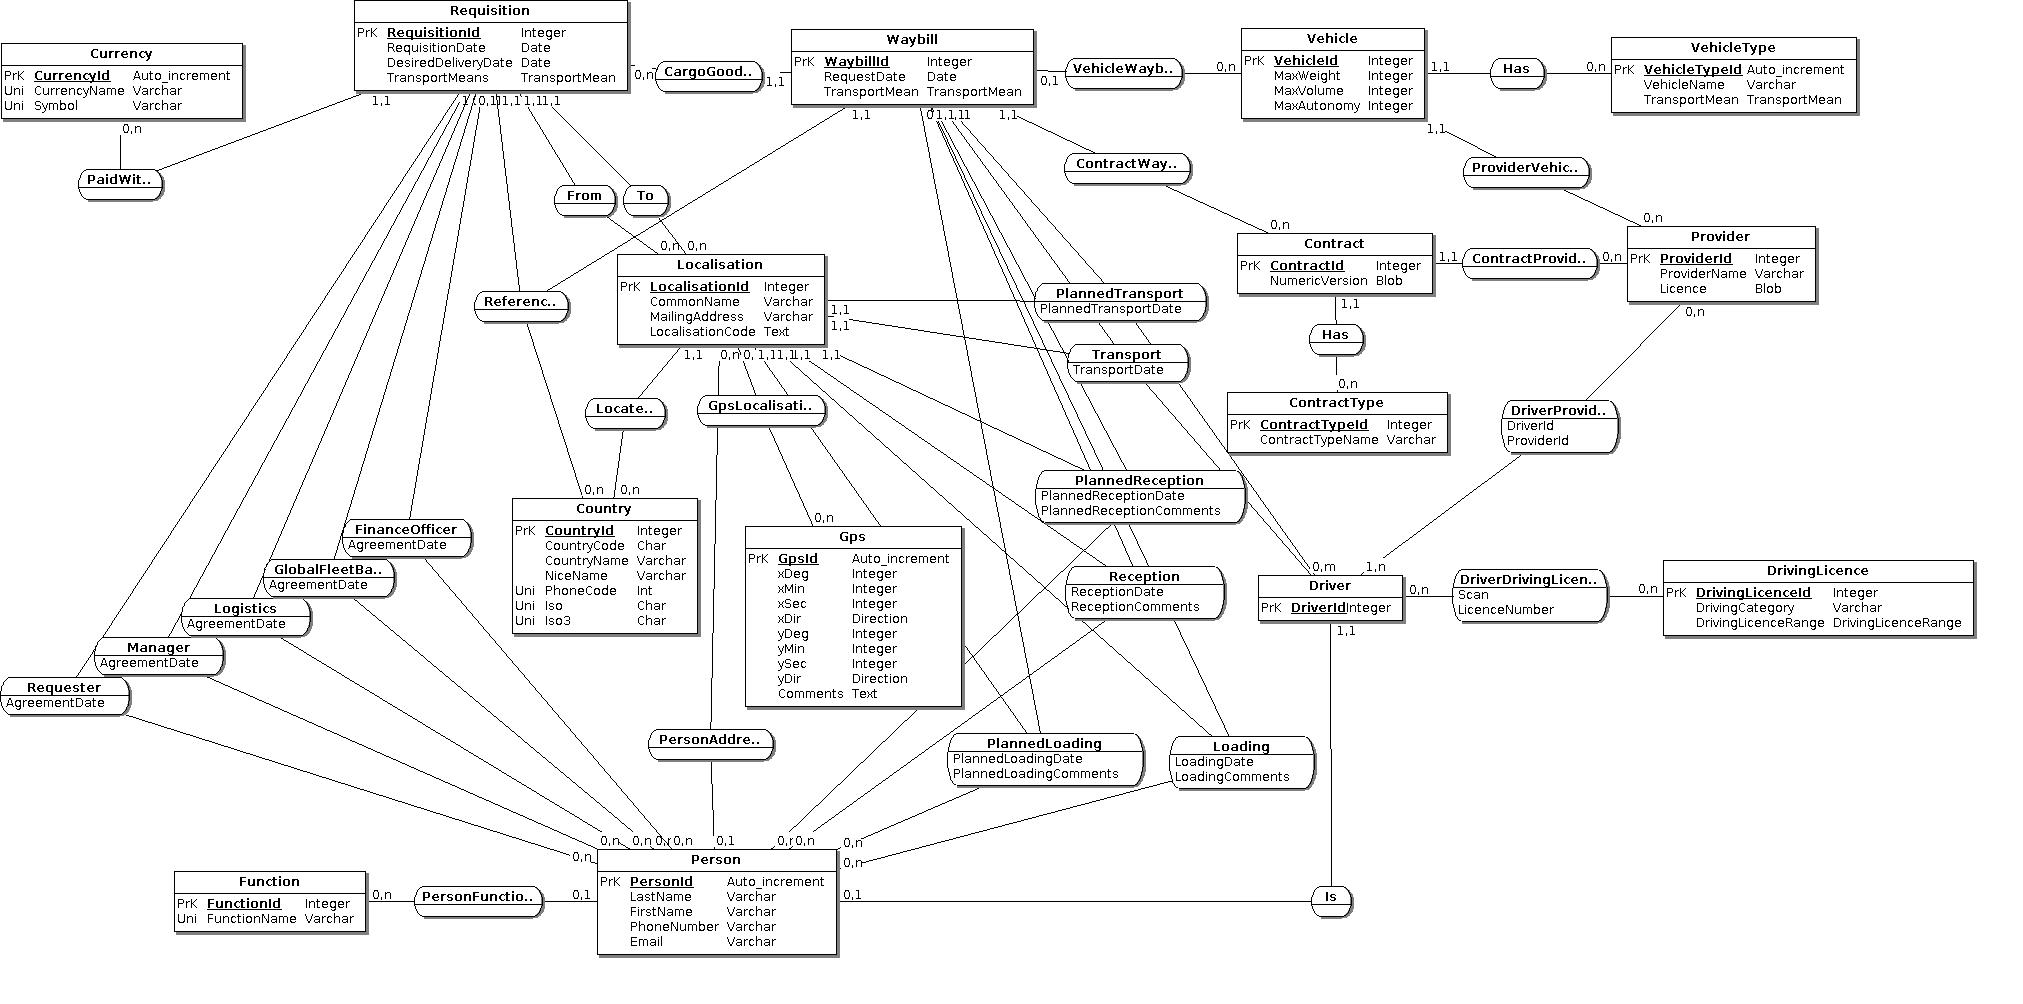
\includegraphics[scale=0.15]{Images/Database}
\end{center}
\end{frame}

\begin{frame}
\frametitle{Implémentation}

\begin{block}{Fonctionnement de la base de données}
Le bon fonctionnement de la base de données s'appuie sur les fichiers suivants~:
\begin{enumerate}
	\item \emph{GkTms.ini}
	\item \emph{GkTms.mcd}
	\item \emph{GkTms.sql}
\end{enumerate}
\end{block}
\end{frame}

\subsubsection[Sauvegarde de secours]{Sauvegarde de secours}
\begin{frame}
\frametitle{Sauvegarde de secours}
\begin{block}{}
Ce SGBDR fournit un outil facile à mettre en place pour la réplications et la sauvegarde des données sur le principe maitre~/~esclave.
\end{block}
\end{frame}

\subsubsection{Difficultés rencontrées}
\begin{frame}
\frametitle{Difficultés rencontrées}
\begin{block}{\textbf{Principaux problèmes}}
\begin{itemize}
\item Besoin immédiat d'un SGBDR fonctionnel
\item Driver QMYSQL pour Qt
\item Migration du SGBDR
\end{itemize}
\end{block}
\end{frame}
